\documentclass[11pt,a4paper]{article}

% ------------------------------------------------------------
% Pacotes (mesmo preâmbulo da proposta, report/report.tex)
% ------------------------------------------------------------
\usepackage[utf8]{inputenc}
\usepackage[T1]{fontenc}
\usepackage[brazil]{babel}
\usepackage{lmodern}
\usepackage{microtype}
\usepackage{amsmath,amssymb}
\usepackage{enumitem}
\usepackage{geometry}
\usepackage{titlesec}
\usepackage{booktabs}
\usepackage{graphicx}
\usepackage{caption}
\usepackage{hyperref}

% ------------------------------------------------------------
% Layout
% ------------------------------------------------------------
\geometry{top=1.8cm, bottom=1.8cm, left=1.9cm, right=1.9cm}

\setlength{\parindent}{0pt}
\setlength{\parskip}{3pt}
\setlist[itemize]{leftmargin=1.35em, itemsep=0.8pt, topsep=2pt, parsep=0pt}
\setlist[enumerate]{leftmargin=1.55em, itemsep=0.8pt, topsep=2pt, parsep=0pt}

\titleformat{\section}{\bfseries\normalsize}{}{0pt}{}
\titlespacing*{\section}{0pt}{7pt}{2pt}

\captionsetup{font=small, labelfont=bf, skip=3pt}
\setlength{\textfloatsep}{8pt}
\setlength{\floatsep}{6pt}
\setlength{\intextsep}{6pt}
\setcounter{topnumber}{3}
\renewcommand{\topfraction}{0.9}
\renewcommand{\textfraction}{0.1}

\hypersetup{colorlinks=true, linkcolor=black, urlcolor=blue}

\newcommand{\repo}{https://github.com/annwith/gender-representation-networks}
\newcommand{\dados}{\repo/tree/main/data/graphml}
\newcommand{\visual}{\repo/blob/main/report/entrega-parcial-visualizacao/entrega-parcial-visualizacao.pdf}
\newcommand{\coleta}{https://annwith.github.io/gender-representation-networks/coleta/}

% ------------------------------------------------------------
% Documento
% ------------------------------------------------------------
\begin{document}

\begin{center}
    {\large\bfseries MO438 -- Redes Complexas: Entrega Parcial (Redes Direcionadas)}\\[2pt]
    Da rede lexical à rede contextual: reorganização das representações
    internas de Transformers com Redes Complexas\\[2pt]
    Juliana Midlej do Espirito Santo (RA 200208)
\end{center}

\vspace{-2mm}

% ============================================================
\section*{1. Introdução}

Na entrada de um Transformer, todas as ocorrências de um mesmo token têm o mesmo
\textit{embedding}; ao atravessar as camadas, essas representações incorporam o contexto e
se reorganizam. O projeto descreve essa transformação como uma sequência de redes complexas
sobre \textbf{os mesmos vértices}: cada vértice é uma \textit{ocorrência} de um token em um
texto, e cada ocorrência aponta para as $k$ ocorrências mais semelhantes a ela. Comparando as
redes camada a camada, medimos quanto a vizinhança deixa de ser determinada pela identidade
do token e passa a refletir o contexto. Esta versão analisa as redes \textbf{direcionadas},
que são o objeto produzido diretamente pelo k-NN.

\textbf{Dados do projeto:} \url{\repo}. As redes estão em
\href{\dados}{\nolinkurl{data/graphml/}}, em GraphML
(\texttt{\textit{rede}\_k10\_directed.graphml}), com os atributos dos
vértices descritos em \nolinkurl{data/graphml/README.md}; os arcos não têm atributos. Esta
versão é gerada por \nolinkurl{scripts/partial_delivery/export_networks.py}, com a opção
\texttt{-{}-sym directed}. A visualização das redes é entregue em um arquivo
separado, \href{\visual}{\texttt{entrega-parcial-visualizacao.pdf}}. A página interativa
\mbox{\url{\coleta}} mostra, passo a passo, como as redes foram construídas.

% ============================================================
\section*{2. Origem dos dados e construção das redes}

As redes são originais, construídas por nós a partir de duas fontes públicas: a
\textbf{Wikipédia em português} (\url{https://pt.wikipedia.org}, CC BY-SA), obtida pela
API MediaWiki a partir de 8 categorias temáticas, com a revisão de cada artigo em
\texttt{data/corpus/manifest.csv}; e o modelo
\href{https://huggingface.co/Qwen/Qwen3-4B-Base}{\textbf{Qwen3-4B-Base}} (36 blocos,
revisão \texttt{906bfd4}), cujo \textit{tokenizer} também define os tokens. Na página interativa,
as abas \href{\coleta}{Rede}, \href{\coleta\#amostra}{Amostra} e
\href{\coleta\#construcao}{Construção} ilustram a coleta, a amostra de vértices e a construção
dos arcos.

\textbf{Coleta.} Em cada tema, uma busca em largura percorre as subcategorias até a
profundidade 2, para em 600 títulos e sorteia 150 artigos. A busca para antes de abrir todas
as subcategorias (de 7 de 79 em computação a 98 de 439 em música), e, como a API as lista em
ordem alfabética, o corte não é aleatório: os temas são ``artigos próximos da categoria
raiz'', e não a área inteira, o que basta para o nosso uso (temas bem separados). Outras 16 categorias ligadas a temas
(profundidade 1, até 60 artigos cada) reforçam sentidos raros das palavras-alvo
(\textit{nota} como cédula, \textit{banco} de areia).

\textbf{Vértices.} Cada vértice é uma \textit{ocorrência}: um token do Qwen3, que pode ser só
um pedaço de palavra, numa posição de um parágrafo. São 13.606 ocorrências de 2.864 tipos de
token, em 3.230 parágrafos de 1.172 artigos (o corpus tem 17.066 parágrafos de 2.153
artigos), com no máximo 50 ocorrências por tipo. O \textbf{núcleo} (10.020
vértices, 74\%) reúne \emph{todos} os tokens de 80 parágrafos sorteados, 10 por tema,
inclusive fragmentos, números e pontuação. Como 80 parágrafos quase não repetem palavras de
conteúdo, três estratos acrescentam palavras inteiras sorteadas em outros parágrafos, nos
quais o resto do texto serve só de contexto: 11 palavras polissêmicas (\textbf{alvos}, 477
ocorrências, com uma cota por tema de sentido, como \textit{banco} em economia, computação e
geografia), 6 palavras sem ambiguidade forte (\textbf{controles}, 277) e 150 palavras
presentes em ao menos 3 temas (\textbf{multitemáticas}, 2.832). Como o núcleo tem três
quartos dos vértices, as medidas globais descrevem sobretudo texto corrido.

\textbf{Vetores.} Cada parágrafo, precedido do separador \texttt{<|endoftext|>}, passa
sozinho pelo Qwen3, sem o título nem os outros parágrafos do artigo. O vetor \textbf{lex} é a
linha do token na matriz de \textit{embeddings}, igual para todas as ocorrências do token;
\textbf{L01}, \textbf{L18} e \textbf{L36} são as saídas brutas (antes da normalização final)
dos blocos 1, 18 e 36, de dimensão 2560, lidas por \textit{hooks} do PyTorch na posição de
cada ocorrência. Como a atenção é causal, o vetor de uma posição depende só do seu token e
dos anteriores.

\textbf{Arcos.} Cada ocorrência $i$ aponta, entre as outras 13.605, de qualquer parágrafo,
artigo ou tema, para as $k=10$ de maior cosseno (calculado em \texttt{float64}) com o
seu vetor $x_i$: $i\to j$ para $j\in N_i$, o conjunto desses vizinhos. A comparação entre
parágrafos diferentes acontece só no espaço dos vetores, e as quatro redes diferem apenas em
$x_i$. Em lex, as ocorrências de um mesmo token são idênticas, e os empates são desfeitos ao
acaso. Os arcos não têm peso: não guardam o valor do cosseno.

% ============================================================
\section*{3. Definições para a rede direcionada}

\textbf{Clusterização (Fagiolo, 2007).} Com $S=A+A^\top$, o número de triângulos
dirigidos que passam por $i$ é $t_i=\tfrac12(S^3)_{ii}$, e o máximo possível é
$D_i=d_i^{\text{tot}}(d_i^{\text{tot}}-1)-2d_i^{\leftrightarrow}$, em que
$d_i^{\text{tot}}=d_i^{\text{in}}+d_i^{\text{out}}$ e $d_i^{\leftrightarrow}$ é o número
de vizinhos recíprocos. A clusterização local é $C_i^{\rightarrow}=t_i/D_i$, definida só
quando $D_i>0$, isto é, quando $i$ tem ao menos 2 vizinhos distintos (aqui, sempre, pois o
grau de saída é 10). Os coeficientes globais são a média $\bar C^{\rightarrow}$ sobre esses
vértices e a transitividade dirigida $T^{\rightarrow}=\sum_i t_i/\sum_i D_i$; com $A$
simétrica, eles se reduzem aos não direcionados.

\textbf{Componentes.} Há duas noções: \textit{fracas}, ignorando o sentido dos arcos (são
as componentes da rede não direcionada), e \textit{fortes}, em que há caminho de $i$ para
$j$ \textbf{e} de $j$ para $i$.

\textbf{Distâncias.} $d(i,j)$ é o número de arcos do menor caminho dirigido de $i$ a $j$;
não é simétrica e vale $\infty$ quando não há caminho. Como nenhuma das redes é fortemente
conexa, a média sobre todos os pares e o diâmetro são $\infty$. Reportamos, com a fração de
pares ordenados que têm caminho, três substitutos finitos: (a) média e máximo só sobre os
pares com caminho; (b) média e diâmetro na maior componente forte; (c) a eficiência global
$E=\frac{1}{|V|(|V|-1)}\sum_{i\neq j}1/d(i,j)$, com $1/\infty=0$, e sua inversa $1/E$.

% ============================================================
\section*{4. Análise inicial}

\begin{table}[h]
\centering
\footnotesize
\setlength{\tabcolsep}{3.5pt}
\caption{Métricas das quatro redes direcionadas ($k=10$). Distâncias exatas, por busca em
largura a partir de cada vértice. As duas últimas linhas comparam as redes; o Jaccard é
$|A\cap A'|/|A\cup A'|$, com $A$ os arcos da rede e $A'$ os da coluna anterior.}
\label{tab:metricas}
\begin{tabular}{lrrrr}
\toprule
Métrica & lex & L01 & L18 & L36 \\
\midrule
Vértices & 13.606 & 13.606 & 13.606 & 13.606 \\
Arcos & 136.060 & 136.060 & 136.060 & 136.060 \\
Grau médio de entrada = de saída & 10 & 10 & 10 & 10 \\
Grau de entrada máximo & 29 & 60 & 55 & 247 \\
Vértices com grau de entrada 0 & 0,7\% & 3,6\% & 0,7\% & 5,4\% \\
Reciprocidade (arcos com arco inverso) & 49,1\% & 57,3\% & 60,7\% & 43,7\% \\
Densidade ($\times 10^{-4}$) & 7,350 & 7,350 & 7,350 & 7,350 \\
Transitividade dirigida $T^{\rightarrow}$ & 0,440 & 0,510 & 0,325 & 0,230 \\
Clusterização local média $\bar C^{\rightarrow}$ & 0,437 & 0,534 & 0,331 & 0,296 \\
Componentes fracas & 44 & 40 & 2 & 2 \\
Componentes fortes & 1.059 & 1.768 & 173 & 1.517 \\
Maior componente forte (vértices) & 2.640 (19,4\%) & 3.862 (28,4\%) & 12.997 (95,5\%) & 10.930 (80,3\%) \\
Pares ordenados com caminho & 17,7\% & 25,4\% & 95,1\% & 80,2\% \\
(a) Distância média entre pares com caminho & 10,37 & 11,28 & 6,97 & 9,96 \\
(a) Maior distância finita & 33 & 39 & 20 & 50 \\
(b) Distância média na maior comp.\ forte & 9,80 & 10,36 & 6,95 & 9,73 \\
(b) Diâmetro da maior comp.\ forte & 30 & 37 & 20 & 50 \\
(c) Eficiência global $E$ & 0,020 & 0,027 & 0,147 & 0,100 \\
(c) Distância harmônica $1/E$ & 49,41 & 36,86 & 6,79 & 9,98 \\
\bottomrule
\end{tabular}

\end{table}

\textbf{Tamanho, grau e densidade.} As quatro redes têm 13.606 vértices e
136.060 arcos. Todo vértice tem grau de saída exatamente $k=10$, então o grau médio de
entrada e de saída é 10, e a densidade $\rho=|A|/(|V|(|V|-1)) = k/(|V|-1) = 7{,}35\times
10^{-4}$ é fixada pela construção. A informação está no grau de entrada $d_i^{\text{in}}$
(quantos escolheram $i$), cuja distribuição (Fig.~\ref{fig:graus-clust}) diferencia as redes:
em lex o máximo é 29; em L36 ele chega a 247, e 5,4\% dos vértices não são escolhidos por
ninguém (\textit{hubness}).

\begin{figure}[h]
\centering
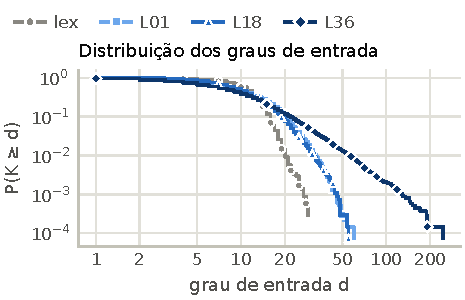
\includegraphics{figuras/graus.pdf}\hfill
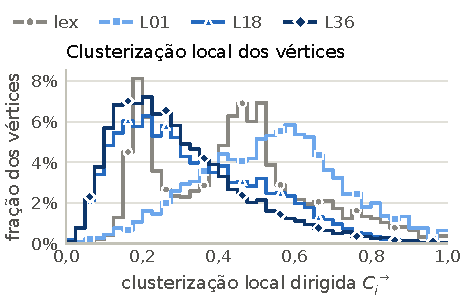
\includegraphics{figuras/clusterizacao_local.pdf}
\caption{À esquerda, a distribuição dos graus de entrada, $P(K\ge d)$ em escala log-log
(item 7). À direita, a da clusterização local dirigida $C_i^{\rightarrow}$ (item 3).}
\label{fig:graus-clust}
\end{figure}

\textbf{Clusterização.} $T^{\rightarrow}$ e $\bar C^{\rightarrow}$ são altas em lex e L01 (0,44--0,53) e menores em L18
e L36 (0,23--0,33). A distribuição de $C_i^{\rightarrow}$ em L18 e L36 se concentra perto de
0,2. Em lex ela tem dois picos (perto de 0,18 e de 0,45).

\begin{figure}[h]
\centering
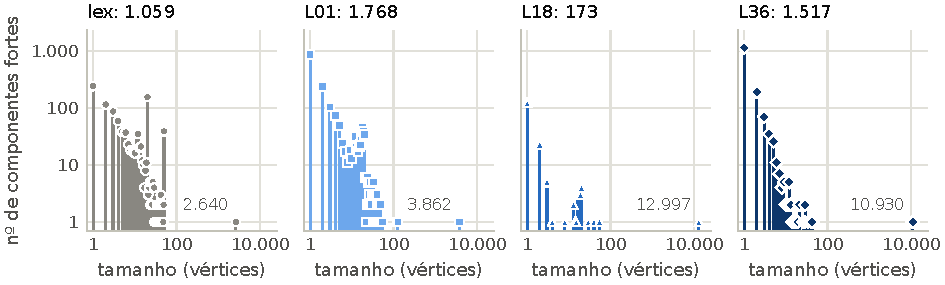
\includegraphics{figuras/componentes.pdf}
\caption{Distribuição dos tamanhos das componentes fortes (item 8; o título dá o número
de componentes e o rótulo, o tamanho da maior).}
\label{fig:componentes}
\end{figure}

\textbf{Componentes (Fig.~\ref{fig:componentes}).} As componentes fortes são muito mais numerosas
(1.059 em lex, 1.768 em L01, 173 em L18 e 1.517 em L36) que as fracas (44, 40, 2 e 2). Em lex, 58\% das ocorrências têm os 10 vizinhos do
próprio token: os grupos de ocorrências de um token frequente apontam só para dentro e
formam ``ralos'' de onde nenhum arco sai (388 componentes, 64\% dos vértices). Em L36, os
tamanhos-1 vêm sobretudo dos vértices que ninguém escolhe.

\begin{figure}[h]
\centering
\begin{minipage}[c]{0.49\textwidth}
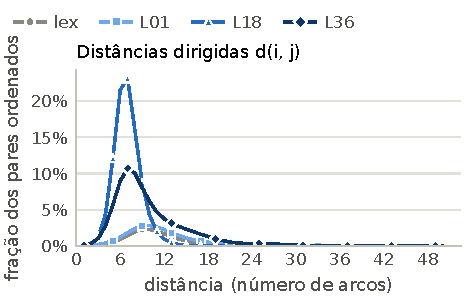
\includegraphics{figuras/distancias.pdf}
\end{minipage}\hfill
\begin{minipage}[c]{0.47\textwidth}
\caption{Distâncias dirigidas (itens 4 e 5): fração de \emph{todos} os pares ordenados a
cada distância finita. A área sob cada curva é a fração de pares com caminho (Tabela~1); os
demais têm $d=\infty$.}
\label{fig:distancias}
\end{minipage}
\end{figure}

\textbf{Distâncias (Fig.~\ref{fig:distancias}).} Os pares sem caminho são
82\% em lex, 75\% em L01, 5\% em L18 e 20\% em L36, e cada substituto distorce a comparação:
(a) compara médias sobre populações diferentes (10,4 em lex, sobre 18\% dos pares, e 7,0 em
L18, sobre 95\%) e não é monótona, pois remover um arco pode \emph{diminuir} a média;
(b) compara subconjuntos diferentes (a maior componente forte de lex tem só 19\% dos
vértices); (c) mistura alcance com distância ($1/E$ dá 49 em lex contra 6,8 em L18,
sobretudo porque lex tem muitos pares sem caminho). Em L36, a maior distância finita chega a
50.

\textbf{Comparação entre as redes.} As duas últimas linhas da Tabela~\ref{tab:metricas}
comparam as redes arco a arco. A fração dos arcos entre ocorrências do mesmo token é de 70\%
em lex e 69\% em L01 e cai para 43\% em L18 e 25\% em L36. O Jaccard com a rede anterior é 0,18 de L01
para L18 e 0,16 de L18 para L36: os arcos mudam tanto entre os blocos 18 e 36 quanto entre os
blocos 1 e 18. Entre lex e L01 (0,32), ele subestima a semelhança: em lex, o desempate sorteia
quais cópias idênticas se ligam.

\textbf{Síntese.} A versão direcionada confirma a reorganização lex/L01 $\to$ L18/L36
(clusterização menor, componente forte gigante, \textit{hubs} em L36) e mostra, arco a arco,
que ela continua entre os blocos 18 e 36. Os grupos fechados por token em lex e os vértices não escolhidos em
L36 deixam muitos pares sem caminho.

\end{document}
